\documentclass[12pt]{article}

\usepackage[letterpaper, hmargin=0.75in, vmargin=0.75in]{geometry}
\usepackage{float}
\usepackage{url}
\usepackage{listings}
\usepackage{graphicx}
\usepackage{courier}

\lstset{basicstyle=\footnotesize\ttfamily}
\pagestyle{empty}

\title{SE465-001\\Assignment 1}
\author{Kevin Carruthers (20463098), {\tt KevinJames@thekev.in}}
\date{February 2, 2015}

\begin{document}

\maketitle

\section*{Question 1}
I found the following results:
\begin{itemize}
\item in {\bf C}: \verb+-5%2+ is -1
\item in {\bf Java}: \verb+-5%2+ is -1
\item in {\bf Perl}: \verb+-5%2+ is 1
\item in {\bf Python}: \verb+-5%2+ is 1
\end{itemize}

The reason for this discrepency is that C-based languages don't use modulus as an operator per-se, rather they use the remainder operator. Java and C, then, report negative values as a result.

\paragraph{Strategy 1.}
We can change the C, Java, etc compilers to return positive results. Something like
\begin{verbatim}
int modulus(int a, int b) {
    return a % b >= 0 ? a % b : (a % b) * -1;
}
\end{verbatim}

\paragraph{Strategy 2.}
We could change the standards of what we expect a modulus to represent to include \emph{equivalence classes}. By definition of modulus arithmetic, for \verb+-5%2+ we have $-1$ and $1$ both in the same equivalence class as the answer (as would be $\dots, -7, -5, -3, 3, 5, 7, \dots$).

\section*{Question 2}

Here are the requested test cases:

\begin{lstlisting}[language=Java]
  public class Question2Tests {
    
    @Test
    public void doesNotExecuteFault() {
      assertThrows(odd({}), NullPointerException());
    }

    public void executesFaultButNoErrorState() {
      assertEquals(odd({1, 2, 3, 4, 5}), 3);
    }

    public void errorButNoFailure() {
      // this is not possible, since any error state (incorrect value of {\tt count})
      // will be output (which makes it a failure as well as an error).
    }
  }
\end{lstlisting}
The first error occurs when an odd negative number ($-9$) is found in the list. The error state is a \verb+count+ which is one lower than it should be (ie. it is still $0$ despite $-9$ being an odd number).


\section*{Question 3}

\paragraph{(a)}
\begin{figure*}[htb]
  \begin{center}
    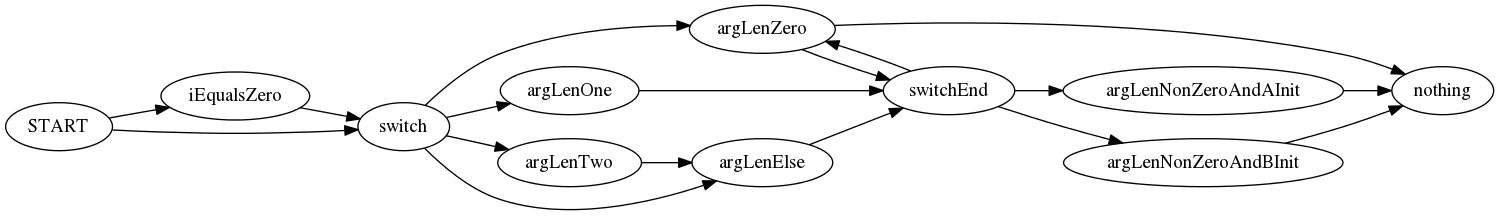
\includegraphics[width=\textwidth]{cfg}
  \end{center}
  \caption{CFG for \ttfamily{M.m()}\rmfamily{}}
\end{figure*}

\paragraph{(b)} Test requirements for various forms of coverage:
\begin{itemize}
  \item $TR_{NC}$: We must hit each node. This can be done by calling the function with an $i == 0$, an {\tt arg} of length zero, an {\tt arg} of length one, and an {\tt arg} of length two or more.
  \item $TR_{EC}$: In this case, edge coverage is equivalent to node coverage (since there are no loops which edge coverage would require we run more than once). See the test cases for $TR_{NC}$ to reach ``full coverage''.
  \item $TR_{EPC}$: Edge-pair coverage requires we visit all edges of length two in our program. Since this is impossible -- because we can not follow paths which require {\tt arg.length()} to be zero to reach the first edge-pair and non-zero for the second -- we can only attempt to ``do our best'': see the test cases for $TR_{EC}$ to get as close as possible.
  \item $TR_{PPC}$: Prime Path coverage requires we cover all paths which are not proper subsets of other paths. This, again, can not give us ``perfect coverage'' for the same reasons as outlined in $TR_{EPC}$. Again, those test requiremments get as as close to prime-path coverage as possible.
\end{itemize}

It is impossible to satisfy any test requirements since each of them require we visit or pass through a node which can only be reached if \verb+argv.length = 0+. Since our main function prohibits this, we can not acheive ``full coverage''.

\section*{Question 4}

\subsection*{Part 1: Test Requirements}
I will test the functions \verb+calculate_maxima()+ and \verb+calculate_raw_allocations()+.

{\bf \verb+calculate_maxima()+.} Test requirements:
\begin{itemize}
\item All of: no accounts and no holdings, no accounts and holdings, accounts and no holdings, accounts and holdings
\item Both of: accounts with \verb+a.can_add_money == True+ and \verb+a.can_add_money == False+
\end{itemize}

{\bf \verb+calculate_raw_allocations()+.} Test requirements:
\begin{itemize}
\item A test case with no allocation rules
\item A test case with a single allocation rules
\item A test case with several equivalent allocation rules
\item A test case with several different allocation rules
\end{itemize}

\subsection*{Part 2: Implementation and Coverage Results}
The coverage report from my tests is below:
\begin{verbatim}
Name                            Stmts   Miss  Cover   Missing
-------------------------------------------------------------
track                               0      0   100%   
track.migrations                    0      0   100%   
track.migrations.0001_initial       5      0   100%   
track.models                       45     41     9%   1-20, 23-26, 29-40,
                                                      43-48, 51-57
track.views                        85     29    66%   74-89, 107-126
-------------------------------------------------------------
TOTAL                             135     70    52%   
-------------------------------------------------------------
\end{verbatim}

\subsection*{Part 3: Fixing a bug; statement coverage}
One of the bugs in {\tt distribute} is {\tt calculate\_maxima}; this function returns {\tt 'N/A'} when {\tt .can\_add\_money} is {\tt True} as opposed to the opposite, which would be expected. This is shown by the test case {\tt testCalculateMaximai()}.

Before the fix:
\begin{verbatim}
======================================================================
FAIL: testCalculateMaxima (track.tests.ViewsTestCase)
----------------------------------------------------------------------
Traceback (most recent call last):
  File "/home/kevin/coding/stqam/a1/q4/distribute/track/tests.py",
      line 57, in testCalculateMaxima
    Account.objects.get(name='acc3'): 345,
AssertionError: Tuples differ:
    ({<Account: acc1 (RRSP)>: (Dec... !=
    ({<Account: acc1 (RRSP)>: (123...

First differing element 0:
{<Account: acc1 (RRSP)>: (Decimal('123'), Decimal('123')),
 <Account: acc2 (TFSA)>: (Decimal('666'), 'N/A'),
 <Account: acc3 (NR)>: (Decimal('345'), 'N/A')}
{<Account: acc1 (RRSP)>: (123, 'N/A'),
 <Account: acc2 (TFSA)>: (666, 666),
 <Account: acc3 (NR)>: (345, 345)}
\end{verbatim}

After the fix:
\begin{verbatim}
OK
\end{verbatim}

I changed line 25 from {\tt if a.can\_add\_money} to {\tt if not a.can\_add\_money}.

This change does not improve test coverage since the lines are executed either way, they simply return incorrect output.

\end{document}
